\documentclass[journal]{IEEEtran}

\ifCLASSINFOpdf
\else
   \usepackage[dvips]{graphicx}
\fi
\usepackage{url}

\hyphenation{op-tical net-works semi-conduc-tor}

\usepackage{graphicx}
\usepackage{hyperref}
\hypersetup{colorlinks=true, linkcolor=blue, urlcolor=cyan}
\usepackage{bm}
\usepackage{mathtools}
\newcommand{\myMatrix}[1]{\bm{\mathit{#1}}}

% Macro to get code font
\def\code#1{\texttt{#1}}


\begin{document}

\title{AMATH 582 Homework 3: Principal Component Analysis}

\author{Eric A. Silk
\thanks{Eric Silk is a Masters Student in Applied Mathematics at the University of Washington,
		and a Research Engineer for Schweitzer Engineering Laboratories, Pullman, WA 99163 (email: esilk16@uw.edu, eric.silk@ericsilk.com)}
}

\markboth{Homework Submission for AMATH 582: Computational Methods for Data Analysis, February 2020}
{Shell \MakeLowercase{\textit{et al.}}: Bare Demo of IEEEtran.cls for IEEE Journals}
\maketitle

\begin{abstract}
Principal Component Analysis (PCA) is a highly useful technique for exploratory data analysis which decomposes a series of observations along axes of the most variance, which then allows for discarding of the less important variables to project into a lower dimensional subspace. This report explores its use in tracking the motion of paint can.
\end{abstract}

\begin{IEEEkeywords}
Singular Value Decomposition, Principal Component Analysis, Object Tracking, OpenCV
\end{IEEEkeywords}


\IEEEpeerreviewmaketitle


\section{Introduction}
\IEEEPARstart{P}{r}incipal Component analysis is a technique used to determine the best method of
representing data in a lower dimensional subspace. It works by using an orthogonal transformation
to convert data which may be correlated into a series of vectors which are uncorrelated. In a 
ense, it can produce the ``best" basis by which to represent a set of data.

In order to explore this method, we will perform PCA upon the motion of a flashlight attached to a
paintcan, moving in a variety of patterns (simple oscillation, oscillation and pendulum motion,
oscillation, pendulum, and spinning), measured by cameras in three arbitrary positions and 
orientations.

\section{Theoretical Background}
\subsection{PCA}
 The technique of Principal Component Analysis works by computing the eigenvalues and eigenvectors
 of the covariance matrix of the data matrix $ \myMatrix{X} $, which is defined as
 $ \myMatrix{X}\myMatrix{X}^{T} $. Calculating this directly can be numerically problematic --
 instead, the Singular Value Decomposition can be used.

 \subsection{SVD}
For full details of the computation, see Dr. Kutz's Book, ``Data-Driven Modeling and Scientific
Computation."

In short, however, SVD of a data matrix produces three matrices:
\begin{equation}
    svd(\myMatrix{X})=\myMatrix{U} \myMatrix{\Sigma} \myMatrix{V}^{*} 
\end{equation}

These resulting matrices can be interpreted within the context of this exercise as follows:
\begin{enumerate}
    \item $\myMatrix{V}$: Each column contains the direction of the PCA modes.
    \item $\myMatrix{\Sigma}$: Singular values on the diagonal, representing the energy of each mode.
    \item $\myMatrix{U}$: Each column represents the displacement in time along a mode
\end{enumerate}

\subsection{Properties}

One of the most important properties of this technique is a relative independence from the bases
used in the initial observation of the data. For instance, in this homework, we are given three
perspectives that are clearly non-orthogonal. Because of our a priori knowledge of the system, we
could conceivably transform the data to force a better perspective. In many cases, this isn't
possible. Use of SVD/PCA will allow us to do this more generally. More importantly, PCA will tell
us which of the modes are most critical in describing the phenomena. This can be used in a number
of ways:

\begin{enumerate}
	\item Data Exploration, to find the "important" modes to investigate further
	\item Feature Engineering, to feed a more limited subset of data to a machine learning algorithm
	\item Visualization, to project a high dimension dataset into a visualizable subspace
	\item Lossy compression, by discarding the lower energy modes
\end{enumerate}

\section{Algorithm Implementation and Development}

\subsection{Object Tracking}

Object tracking proved to be a large portion of the project. In the end, OpenCV with Python
bindings was used to identify and track an object of interest.

\subsubsection{Thresholding}
In order to facilitate object isolation, and given that the paint can had a lit flashlight on top
of it, a simple thresholding of the grayscale image was optionally applied. Specifically, a
``to zero" threshold was used. This works by identifying regions of luminance less than the
threshold and setting them to zero. Comparatively, a binary threshold sets areas below the
threshold to zero and areas above to the maximum luminance. 

\subsubsection{Bounding Box Selection}
The first frame of the video is held on screen until the user draws a bounding box around the
object of interest and presses either the space or enter key. This works quite well in most cases,
except in instances in which the primary point of interest (the lit side of the flashlight) is not
immediately visible.

\subsubsection{Tracking}
Once the bounding box is selected, a tracker provided by OpenCV was used. Specifically, the
\code{CSRT} tracker, or ``Discriminative Filter with Channel and Spatial Reliability" tracker (I'm
unsure how the acronym matches, but alas). This was the best choice in a rather non-rigorous series
of tests, and is touted as a fairly accurate method (albeit more computationally expensive than
some other objects).

One major issue that was noted was, in the event of object occlusion or other loss of tracking,
there was very poor recovery behavior. If this was to be in production, some other method of object
detection would be required, or manual re-selection of the object upon failure.

\subsubsection{Saving of Data}
Upon conversion completion, any failures to track would be recorded as \code{NaN}, and the total
number of these were reported. If the user felt they were acceptable, the data was then saved as
\code{.npy} file for easy import.

\subsection{SVD/PCA}

\subsubsection{SVD}
Fortunately, per instructor permission, the SVD itself was able to be done using a pre-built
implementation. Specifically, \code{numpy.linalg.svd}, which wraps \code{LAPACK}'s \code{\_gesdd}
routine, allowing for high numerical precision and speed.

The observation vectors were stacked before calculating the SVD, truncating to the length of the
shortest for a given case.

\subsubsection{Plotting and Exploration}
Following the example set in Dr. Kutz's book, a series of four plots were made for each case:
\begin{enumerate}
	\item Modal Energy
	\item Modal Energy, on SemiLog axes
	\item Modal behavior of the 2 most significant modes
	\item Temporal behavior of the 2 most significant modes
\end{enumerate}

Additionally, reconstruction of the SVD with only $N$ modes was performed to observe the effects of
discarding lower energy modes.


\section{Computational Results}

\subsection{Kutz Plots}
The results as ``Kutz Plots" (described in ``Plotting and Exploration") for each of the cases can 
be seen in Figures \ref{kutz1}, \ref{kutz2}, \ref{kutz3}, and \ref{kutz4}.

\begin{figure}
	\centerline{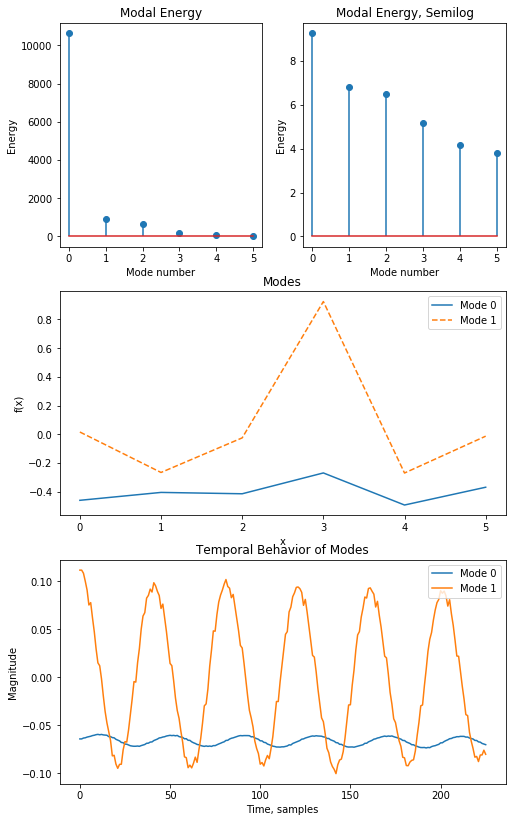
\includegraphics[width=\columnwidth]{kutz1.png}}
	\caption{Kutz Plot, Case 1}
	\label{kutz1}
\end{figure}
\begin{figure}
	\centerline{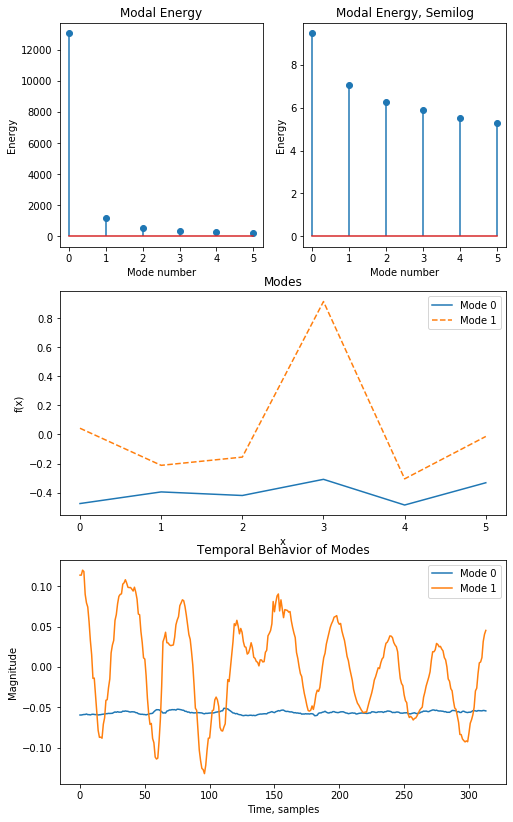
\includegraphics[width=\columnwidth]{kutz2.png}}
	\caption{Kutz Plot, Case 2}
	\label{kutz2}
\end{figure}
\begin{figure}
	\centerline{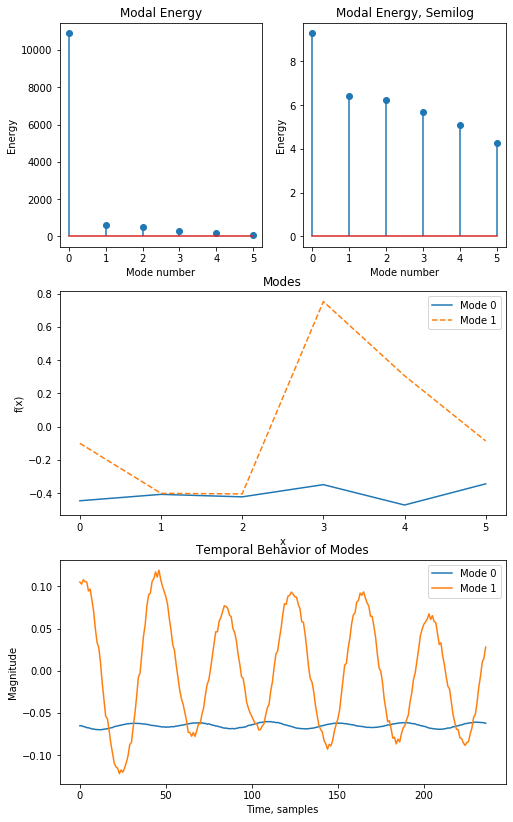
\includegraphics[width=\columnwidth]{kutz3.png}}
	\caption{Kutz Plot, Case 3}
	\label{kutz3}
\end{figure}
\begin{figure}
	\centerline{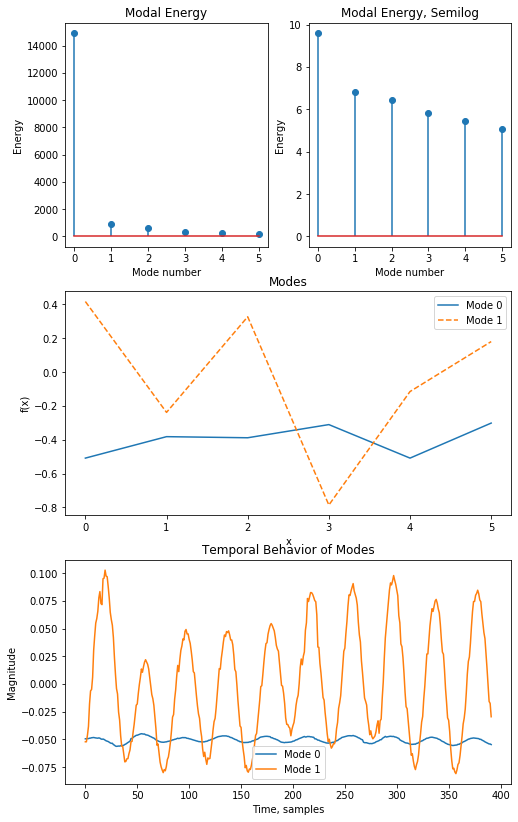
\includegraphics[width=\columnwidth]{kutz4.png}}
	\caption{Kutz Plot, Case 4}
	\label{kutz4}
\end{figure}

The results are a bit confusing. The temporal data indicates that mode zero (the highest energy mode)
demonstrates little change. My best guess is that mode 0 is some offset, since the data hasn't been
normalized to have a mean of zero. Counter to this, however, is that the highest energy mode is
supposed to be the highest variance and thus best at capturing the movement of the paint can; a
roughly constant offset has, by definition, roughly zero variance. Exacerbating the matter, the
second mode appears to demonstrate temporal behavior that matches what is expected -- strongly
oscillatory movement.

The modal data also presents a challenge to parse. Based upon the examples in Dr. Kutz's book, I'm
led to believe this is akin to the basis function for a transform, as evidenced by the example in
figure 160. But, the resulting data doesn't present such a clear function. My assumption is either
that the underlying function is a sinusoid or a somthing like a dirac impulse, which when changed
in time produces the oscillatory behavior of the system.

Encouragingly, both the first and second cases (Fig. \ref{kutz1}, \ref{kutz2}) produce VERY
similar modal results while producing different temporal results. This is indicative of the
ability of the method to ignore the noise introduced by the camera shake.

\subsection{Reconstruction/Projection}
Given that a primary use of PCA is to project the data into a lower subspace, this was explored in
several key plots. For one, the effect of increasing the number of modes was demonstrated in Fig.
\ref{changing_recon}. As expected, more modes show greater complexity of behavior of each time
series. In this case, much beyond two or three modes doesn't appear to improve or change the
resulting plots.
\begin{figure}
	\centerline{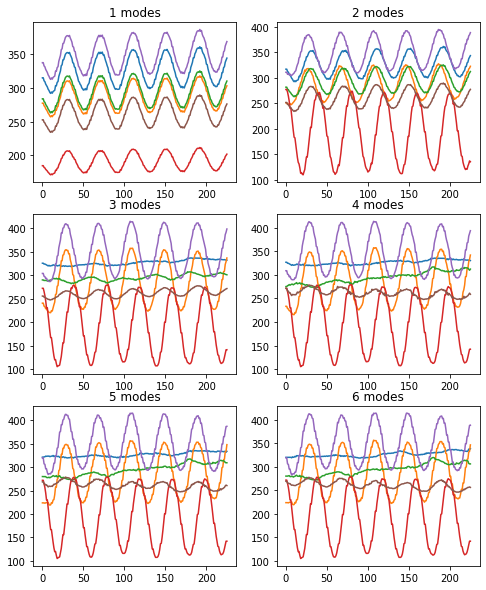
\includegraphics[width=\columnwidth]{changing_recon.png}}
	\caption{Case 1 reconstructed with N modes}
	\label{changing_recon}
\end{figure}

Based upon this threshold, the remaining cases were reconstructed with 3 modes (Figs. \ref{recon2},
\ref{recon3}, \ref{recon4}).
\begin{figure}
	\centerline{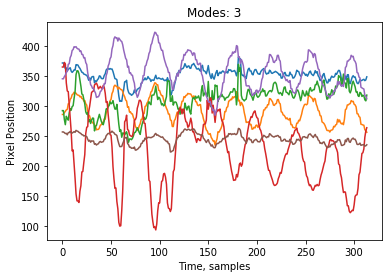
\includegraphics[width=\columnwidth]{recon2.png}}
	\caption{Case 2, Modes=3}
	\label{recon2}
\end{figure}
\begin{figure}
	\centerline{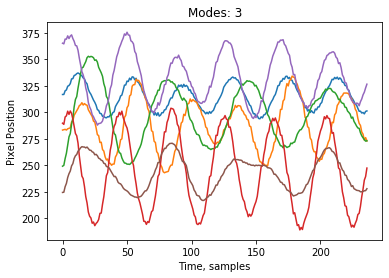
\includegraphics[width=\columnwidth]{recon3.png}}
	\caption{Case 3, Modes=3}
	\label{recon3}
\end{figure}
\begin{figure}
	\centerline{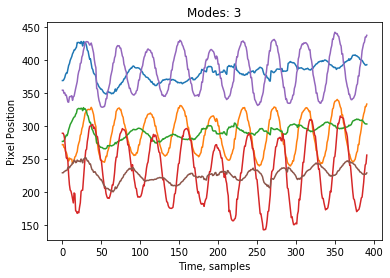
\includegraphics[width=\columnwidth]{recon4.png}}
	\caption{Case 4, Modes=3}
	\label{recon4}
\end{figure}


\section{Summary and Conclusion}


\newpage
\clearpage
\newpage
\section{Appendix A: Functions Used}
\subsection{\code{numpy.lib.stride\_tricks.as\_strided()}}
Given a dataset (1D, in this case), a stride length, and a window width,
return a ``view" into the data. See \href{https://docs.scipy.org/doc/numpy/reference/generated/numpy.lib.stride_tricks.as_strided.html}{here}.


\newpage
\clearpage
\newpage
\section{Appendix B: Python Code}
See my \href{https://github.com/eric-silk/AMATH582_HW3}{Github} for the full repository, including this source code for this IEEE template \LaTeX document. Code is also attached at the end of this report.


\end{document}
